\chapter{Cifras de Fluxo}
\label{cha:cifras-de-fluxo}

No capítulo anterior apresentamos uma definição formal para segurança contra ataques em que o adversário tem acesso apenas ao texto cifrado.
Neste capítulo vamos apresentar uma forma de construir um sistema que satisfaz essa definição.
A ideia geral da construação é a seguinte: partimos de uma sequência aleatória de bits chamado de {\em semente} e a partir dela geramos uma sequência maior de bits a ser usada para encriptar a mensagem usando o ou exclusivo como no OTP.
Apesar desta sequência ser gerada de maneira determinística, a segurança do sistema depende do fato de que ela se pareça aleatória.
Informalmente, um {\em gerador de números pseudoaleatórios} (PRG) é essa função que recebe uma semente aleatória e a expande em uma sequência com cara de aleatória.

Sistemas de cifra de fluxo foram estudados extensamente nos anos 80 \cite{Blum84,Yao82}.
A abordagem para verificar se o gerador de números pseudoaleatórios é suficientemente forte consistia em aplicar uma série de testes estatísticos na sequência gerada para tentar distinguí-lo de uma sequência aleatória.
Assim, por exemplo, um teste pode verificar se a probabilidade de o primeiro bit da sequência ser igual $1$ é $\frac{1}{2}$ ou que a probabilidade de ocorrência de pelos menos três $0$s em qualquer subsequência de tamanho $4$ deve ser $\frac{5}{16}$ -- existem uma sequência em que o $0$ ocorre quatro vezes e mais quatro sequências possíveis em que ele ocorre três vezes.
Um teste recebe uma sequencia produzida por um PRG e deve retornar $1$ se o passar e $0$ se falhar.
O objetivo do teste é distinguir as sequências de bits produzidas por um PRG de uma sequência realmente aleatória.
Por este motivo, esses testes são chamados {\em distinguidores}.

Uma bateria de distinguidores pode ser usada para verificar a qualidade de um PRG.
Idealmente nenhum teste eficiente deveria ser capaz de distinguir o PRG de uma sequência aleatória, ou pelo menos incapaz de fazê-lo com probabilidade considerável\footnote{Usaremos o termo considerável para probabilidades não despreziveis.}.
Definiremos um gerador de números pseudo-aleatórios como um algoritmo $G$ que recebe uma semente $s$ de tamanho $n$ e produz $G(s)$ de tamanho $l(n)$ onde $l$ é um polinômio que define o {\em fator de expansão} do PRG -- quão maior é a sequência produzida em relação a semente -- e tal que nenhum algoritmo polinomial $D$ é capaz de distinguir $G(s)$ de um sequencia $r$ escolhida aleatóriamente em $\{0,1\}^{l(n)}$ com probabilidade não desprezível.
Formalmente temos o seguinte:


\begin{definition}
  Seja $l$ um polinômio e $G$ um algoritmo determinístico polinomial que recebe $s \in \{0,1\}^n$ e retorna $G(s) \in \{0,1\}^{l(n)}$ e seja $r \leftarrow \{0,1\}^{l(n)}$.
  O algoritmo $G$ é um {\em gerador de números pseudo-aleatórios} se:
\begin{enumerate}
\item $l(n) > n$ para todo $n$ e
\item para todo algoritmo polinomial $D$ existe uma função desprezível $\varepsilon$ tal que:
\begin{displaymath}
  |Pr[D(r) = 1] - Pr[D(G(s)) = 1]| \leq \varepsilon(n)  
\end{displaymath}
\end{enumerate}
\end{definition}


\begin{example}
  Considere um algoritmo $G$ que recebe $s \in \{0,1\}^n$ e devolve $0^{l(n)}$.
  Certamente $G$ não é um PRG e podemos mostrar isso com um distinguidor $D$ que recebe $w \in \{0,1\}^{l(n)}$ e devolve $1$ se $w = 0^{l(n)}$ e $0$ caso contrário.
  É fácil ver que para $r \leftarrow \{0,1\}^{l(n)}$ e $s \leftarrow \{0,1\}^n$ temos que $Pr[D(r) = 1] = \frac{1}{2^{l(n)}}$ e $Pr[D(G(s)) = 1] = 1$ e, portanto, temos que:
\begin{displaymath}
  |Pr[D(r) = 1] - Pr[D(G(s)) = 1]| = 1 - \frac{1}{2^{l(n)}}
\end{displaymath}

\end{example}


A restrição de que o distinguidor seja eficiente é extritamente necessária.
Em particular é sempre possível construir um distinguidor usando uma espécie de ataque de força bruta.
Dado uma sequência $w$, o algoritmo $D$ testa todos as possíveis sementes $s$, verifica se $G(s) = w$ e devolve $1$ caso essa semente exista e $0$ se todas falharem.
Esse teste é eficaz pois $Pr[D(G(s)) = 1] =  \frac{1}{2^n}$, mas $Pr[D(r) = 1] = \frac{1}{2^{l(n)}}$ -- existem muito menos sequências em $\{0,1\}^{l(n)}$ geradas por alguma semente do que geradas aleatóriamente.
Porém, o teste não é eficiente.
De fato o tempo esperado para testar todos os valores de $s$ é exponencial, mais precisamente $2^{n-1}$. 

\section{Segurança das Cifras de Fluxo}
\label{sec:streamcipher-sec}

Como adiantamos no capítulo anterior, uma vez definida claramente a suposição que estamos fazendo podemos tentar provar que com essa suposição somos capazes de construir um sistema seguro.
A abordagem para este tipo de prova é uma redução aos moldes das reduções que vimos em Teoria da Computação.
Neste caso vamos reduzir o problema de construir um sistema seguro contra ataques {\em ciphertext only} ao problema de construir um PRG.


\begin{theorem}
\label{theo:stream}
  Se $G$ é um gerador de números pseudo-aleatórios com fator de expansão $l$ então o seguinte sistema $\Pi = \langle Gen, E, D \rangle$ é seguro contra ataques {\em ciphertext only} para mensagens de tamanho fixo $m \in \{0,1\}^{l(n)}$:
\begin{itemize}
\item $Gen(1^n) := k \leftarrow \{0,1\}^n$
\item $E(k,m) = G(k) \xor m$
\item $D(k,c) = G(k) \xor c$
\end{itemize}
\end{theorem}
\begin{proof}
  Seja $\mathcal{A}$ um algoritmo polinomial.
Construiremos um distinguidor $D$ que recebe um string $w \in \{0,1\}^{l(n)}$ e faz o seguinte:
\begin{itemize}
\item Roda $\mathcal{A}(1^n)$ para obter o par de mensagens $m_0, m_1 \in \{0,1\}^{l(n)}$
\item Escolhe $b \leftarrow \{0,1\}$ e computa $c = w \xor m_b$.
\item Entrega $c$ para $\mathcal{A}$ e devolve $1$ se o resultado for igual a $b$ e $0$ caso contrário.
\end{itemize}

Pela definição, $D$ devolve $1$ exatamente nas mesmas situações em que $\mathcal{A}$ vence o desafio.
Portanto temos que:
\begin{displaymath}
Pr[D(G(k)) = 1] = Pr[PrivK^{eav}_{\Pi, \mathcal{A}}(n) = 1]  
\end{displaymath}

Além disso, sendo $\Pi'$ o sistema do OTP e $w \leftarrow \{0,1\}^{l(n)}$ temos que:
\begin{displaymath}
Pr[D(w) = 1] = Pr[PrivK^{eav}_{\Pi', \mathcal{A}}(n)] = \frac{1}{2}  
\end{displaymath}
 
Como $G$ é um PRG temos que existe uma função desprezível $\varepsilon$ tal que $|Pr[D(G(k)) = 1] - Pr[D(w) = 1]| \leq \varepsilon(n)$ e, portanto:
\begin{displaymath}
  |Pr[PrivK^{eav}_{\Pi, \mathcal{A}}(n) = 1] - \frac{1}{2}| \leq \varepsilon(n)
\end{displaymath}

Ou equivalentemente: 
\begin{displaymath}
   Pr[PrivK^{eav}_{\Pi, \mathcal{A}}(n) = 1] \leq \frac{1}{2} + \varepsilon(n)
\end{displaymath}
\end{proof}

Algoritmos validados empiricamente como bons PRG podem ser usados portanto para gerar cifras seguras, ao menos contra ataques {\em ciphertext-only}.
Nos próximos capítulos exploraremos definições mais fortes de segurança e suas respectivas suposições.
Para fechar este capítulo lembramos que as cifras de fluxo sofrem do mesmo problema do OTP quanto à repetição do uso de uma mesma chave.

\section{Modos de Operação}
\label{sec:modos-de-operacao}

Há uma pequena distância entre o resultado do Teorema \ref{theo:stream} e as aplicações práticas das cifras de fluxo da seção \ref{sec:lfsr}, pois o resultado do teorema vale apenas para mensagens de tamanho fixo previamente conhecido.
Em todas situações práticas estamos interessados em criptografar cifras de tamanho arbitrário.
Há duas possíveis soluções para este problema, dois {\em modos de operação} para as cifras de fluxo: síncrono e assíncrono.

Tipicamente, um PRG é formado por um par de algoritmos $\langle Init, GenBits \rangle$.
O primeiro recebe a semente $s$ como entrada e opcionalmente um vetor inicial $IV$ (ver seção seguinte) e devolve um estado inicial $st_0$.
O segundo algoritmo recebe como entrada o estado atual $st_i$, devolve um bit $y$ e atualiza o estado para $st_{i+1}$.
Para cada semente, então, o algoritmo produz um {\em fluxo} de bits -- sendo os $l(n)$ primeiros bits geram $G(s)$.

No modo {\em síncrono} consideramos uma sequência de mensagens $m_0, m_1, \dots$ como uma única grande mensagem $m$.
O algoritmo $Init(s)$ gera o estado inicial $st_0$ e a cada comunicação $GetBits$ parte do estado anterior e gera os bits necessários para encriptar a nova parte da mensagem enviada na comunicação.
A limitação desta abordagem é que as partes precisam mater o estado atual sincronizado, ou seja, quando Alice atualiza $st$, Bob precisa atualizar também.

O outro modo é {\em assíncrono}.
Neste assumimos que além da semente $s$ a algoritmo $G$ recebe uma sequência de bits chamada {\em vetor inicial} $IV$.
O vetor inicial não é sigiloso, mas deve mudar cada vez que uma nova mensagem é criptografada.
Desta forma garantimos que a sequência produzida por $G$ com a mesma chave seja distinta e assim impedimos que ataques de repetição de chaves como mostramos no Capítulo \ref{cha:sigilo-perfeito}.

% CITAR OS ARTIGOS QUE APRESENTAM O TRIVIUM, O RC4 E O ATAQUE CONTRA O WEP

\begin{example}
O Wired Equivalent Privacy (WEP) era o padrão para segurança em conexões WiFi desde 97 e é essencialmene uma cifra de fluxo que opera de modo assíncrono.
Para gerar um fluxo de bits pseudo-aleatórios o WEP utiliza o RC4 \cite{Rivest16} -- um PRG proposto por Ron Rivest em 87 -- que recebe como entrada a semente de 40 ou 104 bits e um vetor inicial não sigiloso de 24 bits.
Para cada pacote transimitido, o WEP gera um novo $IV$ e utiliza a mesma chave para criptografar seu conteúdo.
Acontece que 24 bits é um tamanho consideravelmente pequeno e se repete com 50\% de chance a cada 5000 pacotes tornando-o completamente inseguro \cite{Fluhrer01}.

Hoje em dia, um script que implementa este tipo de ataque chamado {\tt aircrack-ng}\footnote{http://www.aircrack-ng.org/} é capaz de quebrar uma senha WEP usando uma computador pessoal em questão de minutos.
Esse tipo de vulnerabilidade do protocolo WEP levou-o a ser substituído em pelo protocolo WPA e em seguida pelo WPA2 entre 2004 e 2006.
\end{example}

\section{Construções Práticas}
\label{sec:construcoes-praticas}

A existência de PRGs não foi demonstrada matematicamente.
No Apêndice \ref{cha:owf} mostraremos porque é tão difícil encontrar uma PRG demonstradamente seguro.
O importante por enquanto é que é difícil demonstrar a segurança de um sistema e, portanto, a abordagem utilizada em relação a PRG é empírica.
Ou seja, os candidatos a PRG são empiricamente validados a cada tentativa frustrada de construir um distinguidor para eles.


\subsection{Linear-Feedback Shift Registers}
\label{sec:lfsr}

Uma classe de exemplos deste tipo de algoritmo são os chamados {\em Linear-Feedback Shift Registers} (LFSRs).
Um LFSR consiste de um vetor de registradores $s_{n-1} \dots s_0$, que guardam exatamente um bit cada, e uma sequência de bits $c_{n-1} \dots c_0$ chamada {\em coeficientes de feedback}.
A cada passo o estado é atualizado deslocando todo vetor uma posição para a direita e produzindo um novo bit que é calculado como
\begin{displaymath}
s_{n-1} := \bigoplus_{i=0}^{n-1}c_is_i  
\end{displaymath}

\begin{example}
  Considere um LFSR com quatro registradores sendo o primeiro e o terceiro parte do coeficiete de feedback.
Se a configuração inicial dos registradores é $\langle 0,0,1,1 \rangle$ os próximos passos são os seguintes:
\begin{displaymath}
  \langle 0,0,1,1 \rangle \vdash
  \langle 1,0,0,1 \rangle \vdash 
  \langle 1,1,0,0 \rangle \vdash
  \langle 1,1,1,0 \rangle \vdash
  \langle 1,1,1,1 \rangle
\end{displaymath}
\end{example}

Um LSFR com $n$ registradores é capaz de gerar no máximo $2^n$ bits até começar a repetir sua sequência.
Bons LFSR são aqueles que geram a maior quantidade de bits antes de começar a repetir -- essa quantidade de bits é chamada de {\em tamanho do ciclo}.

O segredo do LFSR, sua ``chave'', é a semente $s_{n-1} \dots s_0$ -- lembrem que assumimos que o mecanismo (neste caso os coeficiente de feedback) são sempre conhecidos. 
Um ataque relativamente simples a um LFSR consiste em observar os $n$ primeiros bits gerados $y_{n+1} \dots y_{2n}$ e resolver o seguinte sistema linear:

\begin{eqnarray*}
  y_{n+1} &    =   & c_{n-1}y_n \xor \dots \xor c_0 y_1\\
         & \vdots &  \\
  y_{2n}  &    =   & c_{n-1}y_{2n-1} \xor \dots \xor c_0 y_n\\      
\end{eqnarray*}


É possível mostrar que essas equações são linearmente independentes e, portanto, elas determinam unicamente os coefientes.
Uma vez determinados os valores $y_0 \dots y_n = s_0 \dots s_n$, podemos prever cada novo bit da sequência.
Com isso torna-se simples a tarefa de construir um distinguidor para o gerador.

Resumindo, o LFSR não é seguro pois a operação que gera novos bits é linear, o que permite que ela seja previsível.
LFSRs não são PRG seguros, mas muitos PRGs nada mais são do que versões alteradas deste esquema geral.
Tipicamente os PRGs usados na prática substituem a operação de ou exclusivo por alguma operação não linear.

\subsection{Trivium}
\label{sec:trivium}

Em um concurso científico de 2008 para produção de cifras de fluxo seguras, uma série de algoritmos foram apresentados como alternativas seguras e eficientes para este problema.
Um dos algoritmos selecionados pelo projeto eSTREAM é o {\em Trivium} \cite{DeCanniere06}.
Este algoritmo recebe dois valores como entrada ambos com 80 bits, a semente e o vetor incial.
Um estado no Tivium é um vetor com 288 bits e seu ciclo tem tamanho $2^{64}$, ou seja, $Triv: \{0,1\}^{80}\times \{0,1\}^{80} \to \{0,1\}^{2^{64}}$.

O Trivium possui três registradores A, B e C de tamanhos de 93, 84 e 111 respectivamente, somando 288 bits.
Em cada passo cada registrador:
\begin{enumerate}
\item calcula o AND do penúltimo com o ante-penúltimo bit e calcula o XOR do bit resultante com o último bit e com mais um bit de uma certa posição fixa chamado {\em feedfoward bit} para produzir um bit chamado {\em bit de saída},
\item o bit de saída é enviado para o registrador adjacente -- A envia para B, B para C e C para A,
\item cada registrador move seus bits uma posição para a direita, como no LFSR,
\item cada registrador aplica o XOR do bit que recebeu com um bit de uma certa posição fixa, chamado {\em feedbackward bit}, e insere bit resultante na primeira posição e, por fim,
\item calcula-se o XOR dos três bits de saída para produzir um bit do fluxo.
\end{enumerate}

A chave do Trivium é inserida nas primeiras posições do registrador A, e o vetor inicial nas úlitmas posições do registrador B.
As demais posições são preenchidas com $0$ excetos as últimas três do registrador C que são preenchidas com $1$.
Antes de começar a produzir o fluxo de bits, o processo roda $4 \times 288 = 1152$ no que é chamado de {\em fase de aquecimento}. 
Até a escrita destas notas, não existem ataques conhecidos ao algoritmo mais eficientes do que o ataque de força-bruta.


\begin{figure}
  \centering
  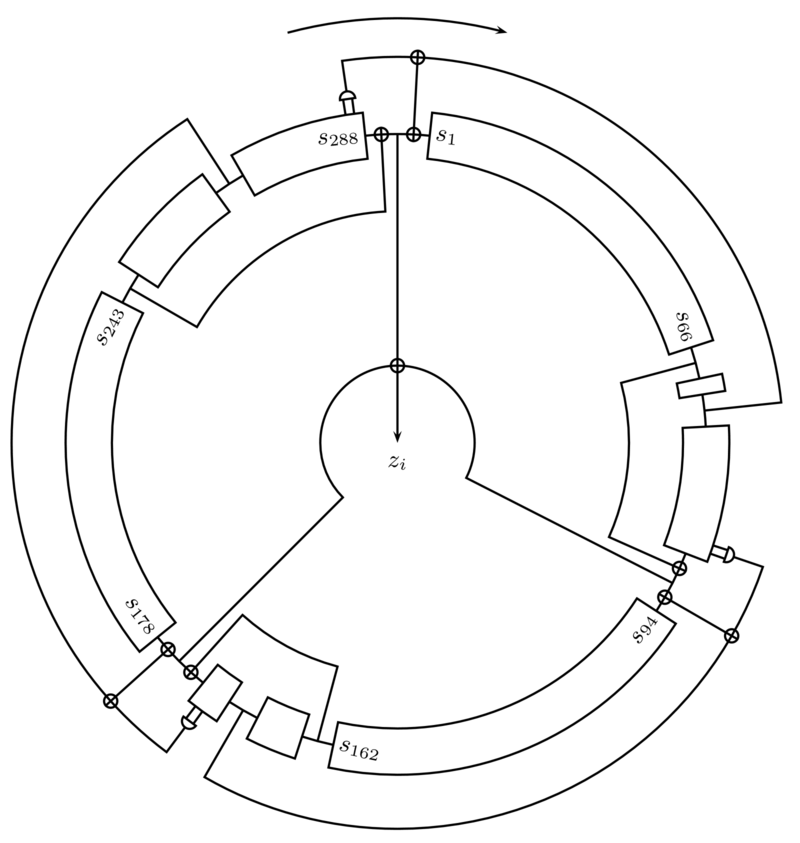
\includegraphics[width=.5\textwidth]{imagens/trivium.png}
  \caption{Estrutura circular do Trivium}
\end{figure}


A escolha de um bom gerador de números pseudo-aleatórios é central para a segurança de uma cifra de fluxo.
Um erro típico é utilizar funções padrão, como a função {\tt rand} da biblioteca padrão do {\tt C}, que não são adequadas para aplicações de segurança.
A orientação geral é buscar os geradores selecionados pelo projeto eSTREAM como o Trivium mencionado nesta seção ou o SALSA20.


\section{Exercicios}
\label{sec:exercicios}

\begin{exercicio}
  O que precisamos assumir para que um sistema de criptografia baseado em cifra de fluxo seja seguro?

  Em que sentido podemos considerá-lo seguro?
\end{exercicio}

\begin{exercicio}
Mostre que o gerador $G$ com fator de expansão $l(n) = n + 1$ que recebe $s \in \{0,1\}^n$ e devolve $s$ concatenado com $\bigoplus_{i=0}^ns_i$ não é um PRG.  
\end{exercicio}

\begin{exercicio}
  Construa um dintinguidor eficiente $D$ para o LFSR simples.
\end{exercicio}

\begin{exercicio}
  Por que em uma cifra de fluxo não podemos criptografar duas mensagens distintas com a mesma chave?
\end{exercicio}

\begin{exercicio}
 Sejam $y_0, y_1, y_2 \dots$ os bits gerados pelo algoritmo RC4.
É possível mostrar que para uma distribuição uniforme de sementes e vetores iniciais, a probabilidade dos bits $y_9, \dots, y_{16}$ serem todos iguais a $0$ é $\frac{2}{256}$.
Mostre como construir um algoritmo eficiente $D$ capaz de distinguir as sequências de bits produzidas pelo RC4 de uma sequência realmente aleatória.
\end{exercicio}

\begin{exercicio}
  Considere a seguinte implementação de uma cifra de fluxo:
\begin{enumerate}
\item Utilizamos o número de segundos desde primeiro de janeiro de 1970 até o momento atual para gerar uma semente $s$ que armazenamos em um local seguro.
\item Utilizamos, então, a implementação {\tt rand} da biblioteca padrão do {\tt C} para gerar uma sequência de $n$ bits $G(s)$.
\item Produzimos a cifra $c = G(s) \xor m$ supondo que $|m| = n$.
\item Para descriptografar recuperamos $s$, aplicamos $G(s) \xor c$.
\end{enumerate}

  Descreva duas vulnerabilidades deste protocolo.
\end{exercicio}


